% Exact square-index subsequence: n_2=4,n_3=9,n_4=16,n_5=25.
% Gaps in sample size are respectively 5,7,9; (n_{k+1}-n_k)/n_k -> 0.
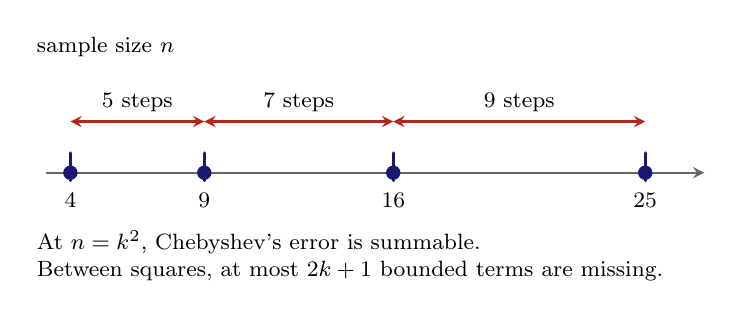
\begin{tikzpicture}[x=1cm,y=1cm,line cap=round,>=stealth]
  \node[font=\footnotesize,anchor=west] at (0,2.0) {sample size $n$};
  \draw[->,black!60,thick] (0.25,0.4)--(8.6,0.4);
  \foreach \x/\val in {0.55/4,2.25/9,4.65/16,7.85/25}{
    \draw[MidnightBlue,very thick] (\x,0.3)--(\x,0.65);
    \fill[MidnightBlue] (\x,0.4) circle (2.6pt);
    \node[below,font=\footnotesize] at (\x,0.26) {$\val$};
  }
  \draw[BrickRed,thick,<->] (0.55,1.05)--(2.25,1.05);
  \draw[BrickRed,thick,<->] (2.25,1.05)--(4.65,1.05);
  \draw[BrickRed,thick,<->] (4.65,1.05)--(7.85,1.05);
  \node[above,font=\footnotesize] at (1.4,1.05) {$5$ steps};
  \node[above,font=\footnotesize] at (3.45,1.05) {$7$ steps};
  \node[above,font=\footnotesize] at (6.25,1.05) {$9$ steps};
  \node[font=\footnotesize,anchor=west] at (0,-0.48) {At $n=k^2$, Chebyshev's error is summable.};
  \node[font=\footnotesize,anchor=west] at (0,-0.85) {Between squares, at most $2k+1$ bounded terms are missing.};
\end{tikzpicture}
